\documentclass[12pt, titlepage]{article}

\usepackage{fullpage} %full page typesetting
\usepackage{setspace} %allows for non-singlespacing
\usepackage{graphicx} %graphics capabilities
\usepackage{latexsym} %extra symbols
\usepackage{rotating} %rotation for figures
\usepackage{longtable} %tables that fill more than a single page
%\usepackage{hyperref} %hypertext links in the document
\usepackage{natbib} %better bibliographies
\usepackage{authblk} %author and affiliation in opening
\usepackage{mathpazo} %use palatino font, rather than times
\usepackage{appendix}
\usepackage{lscape}
\usepackage{tabulary}
\usepackage[nottoc]{tocbibind}
\usepackage[colorlinks=true,linkcolor=blue,citecolor=cyan]{hyperref}
\usepackage{ifthen}
\usepackage{float}
\usepackage{subcaption}
\usepackage{mwe}
\usepackage{caption}
\usepackage{listings}
\lstset{
	basicstyle=\small\ttfamily,
	columns=flexible,
	breaklines=true
}


\title{\tb{Place of Residence and Political Attitudes in Democracies Worldwide \\ {\large Online Appendix C -- Margins Plots} }}

\author{Jennifer Lin}
\affil{New College of Florida}

\newcommand\e{\emph}
\newcommand\tb{\textbf}
\newcommand\un{\underline}
\newcommand\txt{\texttt}

\doublespacing 

\begin{document}

\begin{singlespace}
\maketitle
\end{singlespace}

\section{The Regressions}

The regressions for this model are based on the worldwide trends to better understand how a regime's level of democracy, electoral formula and regime age influence the relationship of the people's place of residence and political attitudes. In addition to these macro variables of interest in the third hypothesis of the main paper, the country's Freedom House rating and Corruption Perception Index score were also added as a means to understanding whether these factors influence the key independent and dependent variables in the analysis.

The following codes were used to run the regressions in Stata Version 15.1. Each variable name is not exactly to what was used due to renames and recodes after the data cleaning process. The variable names included throughout all appendices are used to aid in understanding of the process and connecting the variables used to their descriptions in the CSES Module IV codebook.

\begin{lstlisting}
*Interaction with Place and Democracy
reg ideology i.place##i.democracy regimeage electformula freedomhouse corrupt gender age ses education partyid close religion
rvfplot
margins, dydx(place) at(democracy=(8(1)10))
marginsplot
graph export "IdeoPlaceDem.pdf", replace

reg liberalism i.place##i.democracy regimeage electformula freedomhouse corrupt gender age ses education partyid close religion
rvfplot
margins, dydx(place) at(democracy=(8(1)10))
marginsplot
graph export "LibPlaceDem.pdf", replace

*Interaction with Place and Regime Age
reg ideology i.place##c.regimeage electformula democracy freedomhouse corrupt gender age ses education partyid close religion
rvfplot
margins, dydx(place) at(regimeage=(0(25)200))
marginsplot
graph export "IdeoPlaceAge.pdf", replace

reg liberalism i.place##c.regimeage electformula democracy freedomhouse corrupt gender age ses education partyid close religion
rvfplot
margins, dydx(place) at(regimeage=(0(25)200))
marginsplot
graph export "LibPlaceAge.pdf", replace

*Interaction with Place and Electoral Formula
reg ideology i.place##i.electformula regimeage democracy freedomhouse corrupt gender age ses education partyid close religion
rvfplot
margins, dydx(place) at(electformula=(1 2 3))
marginsplot
graph export "IdeoPlaceFormula.pdf", replace

reg liberalism i.place##i.electrformula regimeage democracy freedomhouse corrupt gender age ses education partyid close religion
rvfplot
margins, dydx(place) at(electofrmula=(1 2 3))
marginsplot
graph export "LibPlaceFormula.pdf", replace

*Interaction with Place and Freedom House Rating
reg ideology i.place##c.freedomhouse electformula regimeage democracy corrupt gender age ses education partyid close religion
rvfplot
margins, dydx(place) at(freedomhouse=(4(.5)7))
marginsplot
graph export "IdeoPlaceFree.pdf", replace

reg liberalism i.place## c.freedomhouse electformula regimeage democracy corrupt gender age ses education partyid close religion
rvfplot
margins, dydx(place) at(freedomhouse=(4(.5)7))
marginsplot
graph export "LibPlaceFree.pdf", replace

*Interaction with Place and Corruption
reg ideology i.place##c.corrupt freedomhouse electformula regimeage democracy gender age ses education partyid close religion
rvfplot
margins, dydx(place) at(corrupt=(0(10)100))
marginsplot
graph export "IdeoPlaceCorrupt.pdf", replace

reg liberalism i.place##c.corrupt freedomhouse electformula regimeage democracy gender age ses education partyid close religion
rvfplot
margins, dydx(place) at(corrupt=(0(10)100))
marginsplot
graph export "LibPlaceCorrupt.pdf", replace
\end{lstlisting}

\section{The Margins Plots}

\begin{figure}[H]
	\centering
	\begin{subfigure}[b]{0.475\textwidth}   
		\centering 
		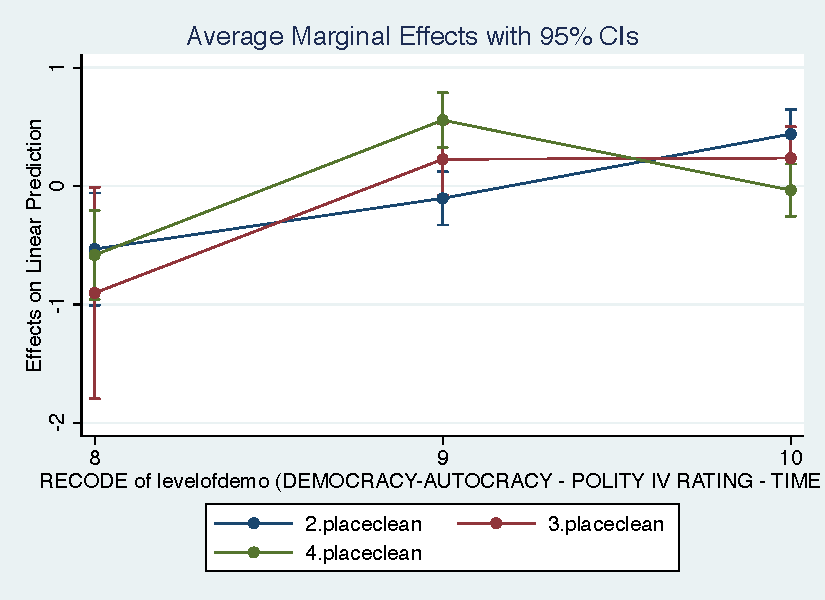
\includegraphics[width=\textwidth]{Margins/IdeoPlaceDem}
		\caption{Self-Placement Ideology}
	\end{subfigure}
	\hfill
	\begin{subfigure}[b]{0.475\textwidth}
		\centering 
		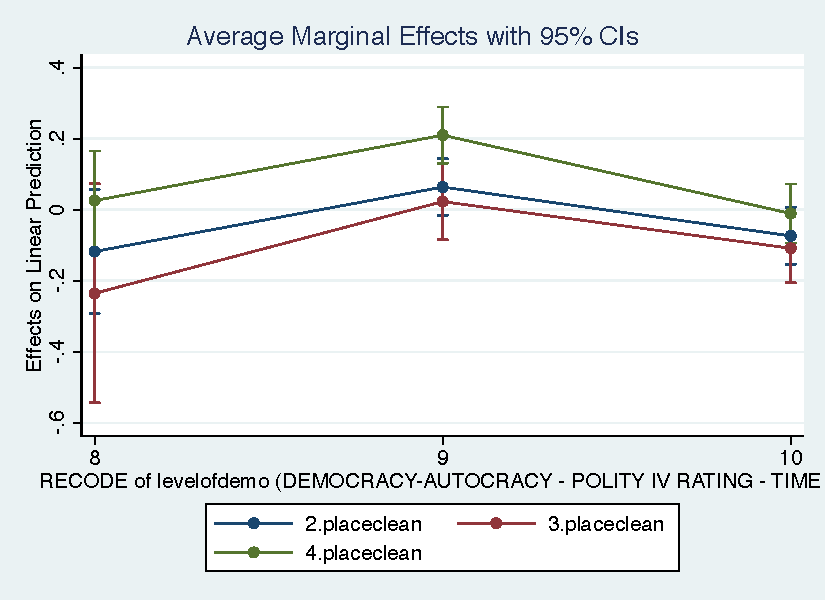
\includegraphics[width=\textwidth]{Margins/LibPlaceDem}
		\caption{Issue Stances}
	\end{subfigure}
	\caption{Margins Plots for Place Interaction with Democracy}
	\label{Democracy}
\end{figure}

\begin{figure}[H]
	\centering
	\begin{subfigure}[b]{0.475\textwidth}   
		\centering 
		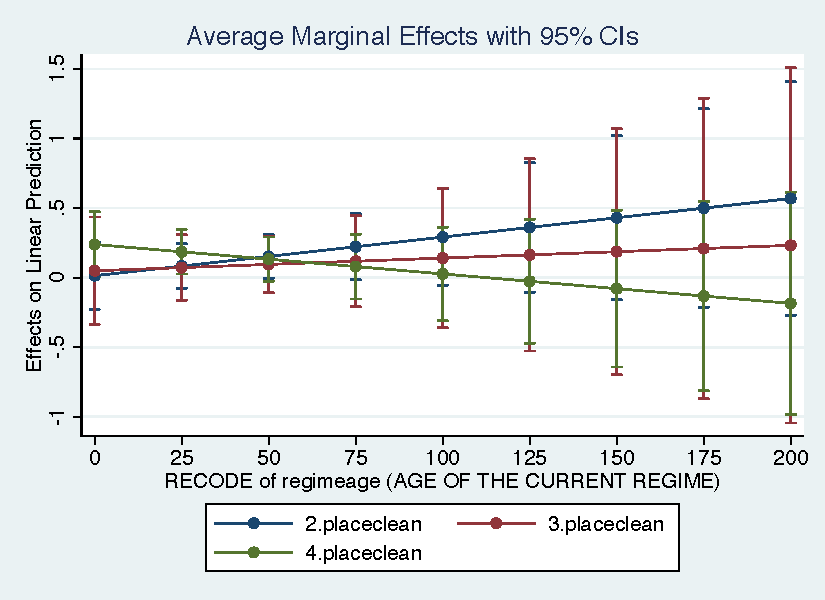
\includegraphics[width=\textwidth]{Margins/IdeoPlaceAge}
		\caption{Self-Placement Ideology}
	\end{subfigure}
	\hfill
	\begin{subfigure}[b]{0.475\textwidth}
		\centering 
		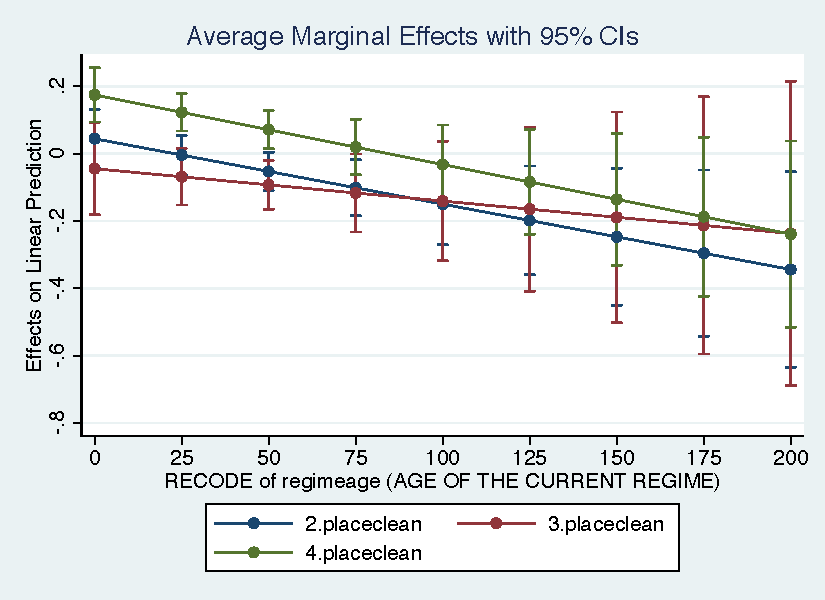
\includegraphics[width=\textwidth]{Margins/LibPlaceAge}
		\caption{Issue Stances}
	\end{subfigure}
	\caption{Margins Plots for Place Interaction with Regime Age}
	\label{Age}
\end{figure}

\begin{figure}[H]
	\centering
	\begin{subfigure}[b]{0.475\textwidth}   
		\centering 
		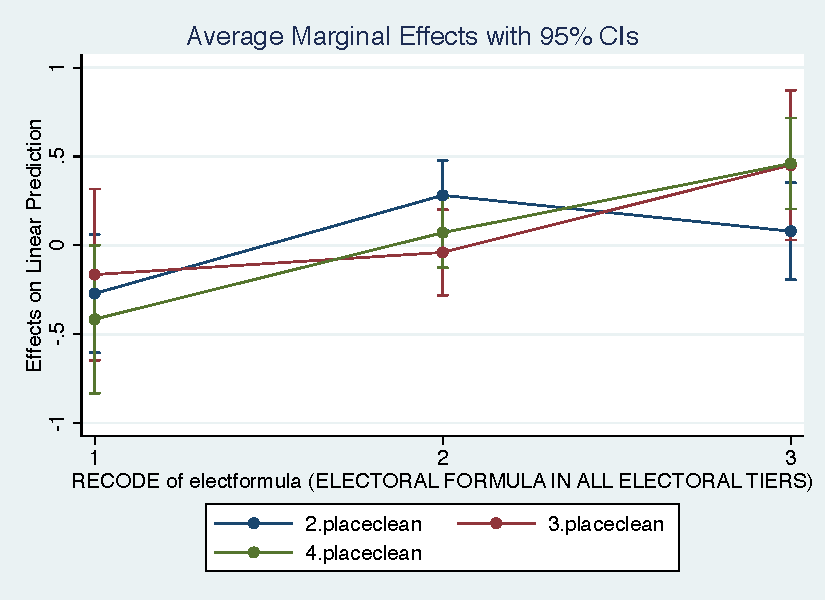
\includegraphics[width=\textwidth]{Margins/IdeoPlaceFormula}
		\caption{Self-Placement Ideology}
	\end{subfigure}
	\hfill
	\begin{subfigure}[b]{0.475\textwidth}
		\centering 
		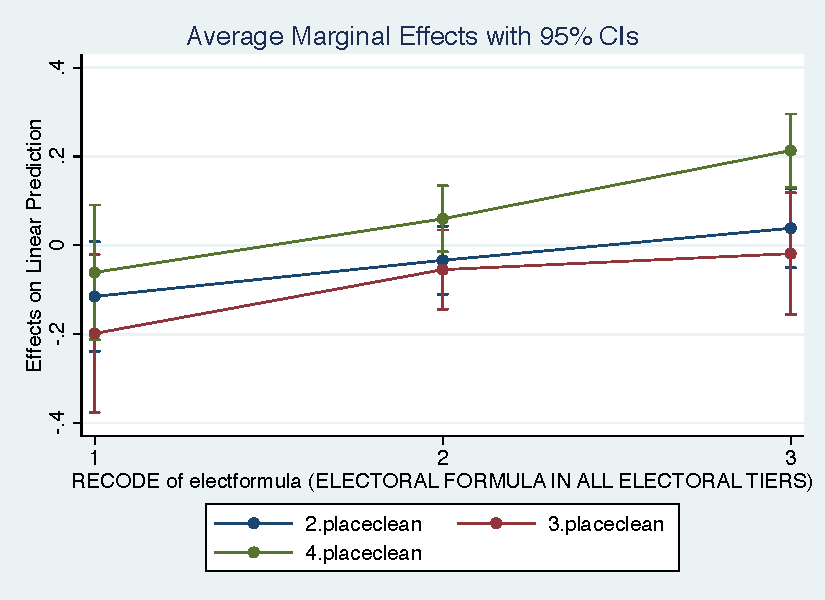
\includegraphics[width=\textwidth]{Margins/LibPlaceFormula}
		\caption{Issue Stances}
	\end{subfigure}
	\caption{Margins Plots for Place Interaction with Electoral Formula}
	\label{Elect}
\end{figure}

\begin{figure}[H]
	\centering
	\begin{subfigure}[b]{0.475\textwidth}   
		\centering 
		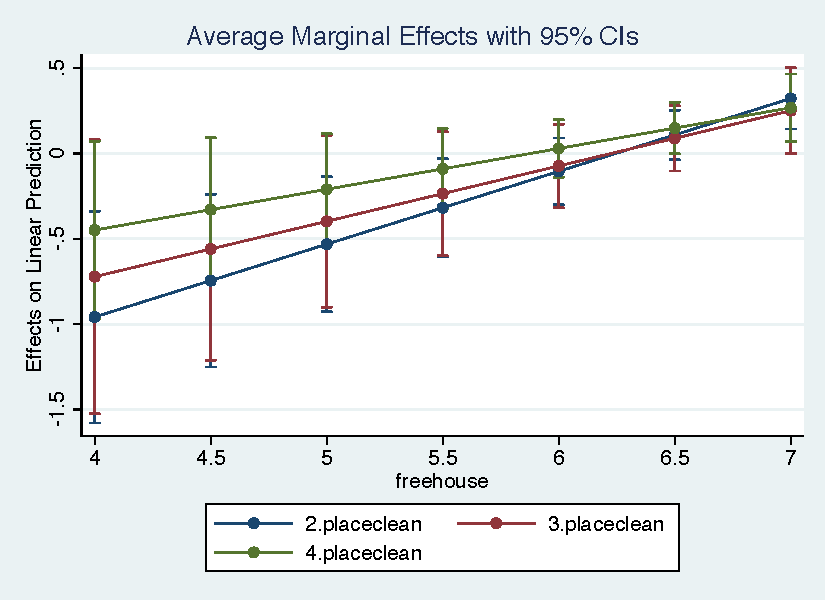
\includegraphics[width=\textwidth]{Margins/IdeoPlaceFree}
		\caption{Self-Placement Ideology}
	\end{subfigure}
	\hfill
	\begin{subfigure}[b]{0.475\textwidth}
		\centering 
		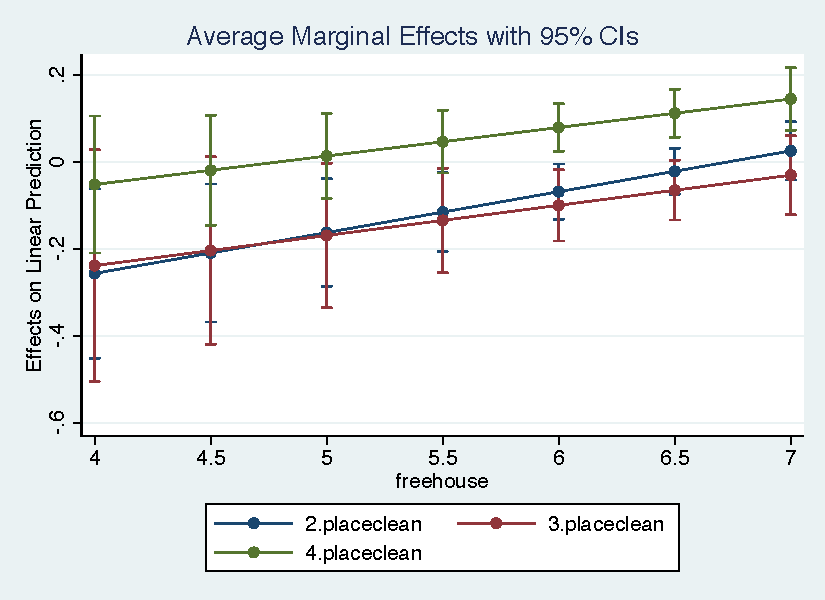
\includegraphics[width=\textwidth]{Margins/LibPlaceFree}
		\caption{Issue Stances}
	\end{subfigure}
	\caption{Margins Plots for Place Interaction with Freedom House Ratings}
	\label{Freedom}
\end{figure}

\begin{figure}[H]
	\centering
	\begin{subfigure}[b]{0.475\textwidth}   
		\centering 
		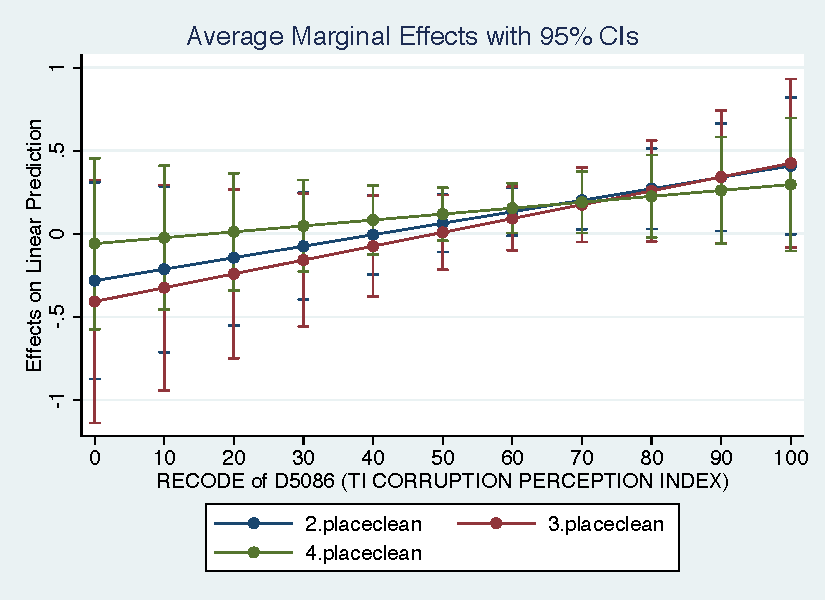
\includegraphics[width=\textwidth]{Margins/IdeoPlaceCorrupt}
		\caption{Self-Placement Ideology}
	\end{subfigure}
	\hfill
	\begin{subfigure}[b]{0.475\textwidth}
		\centering 
		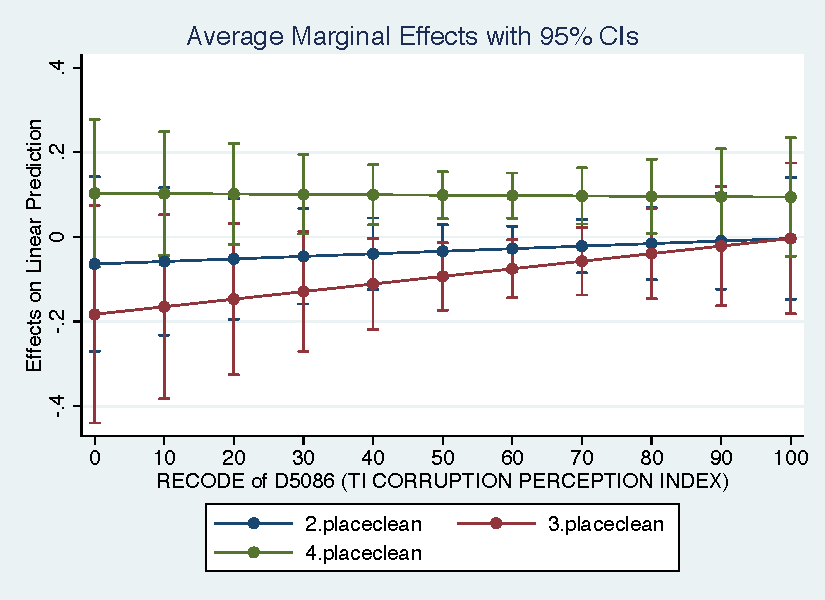
\includegraphics[width=\textwidth]{Margins/LibPlaceCorrupt}
		\caption{Issue Stances}
	\end{subfigure}
	\caption{Margins Plots for Place Interaction with Corruption Perception Index Scores}
	\label{Corruption}
\end{figure}

\end{document}